\chapter{Group by language groups}

\section{Language groups}
1 to 2, 3, 4, 5, etc. models on en-to-36 dataset (0.9 mil. sentences per target language)
compared with random runs
\subsection{Germanic group}
\label{subsection:germanic_group}

Here Germanic group consists of German, Dutch, Swedish, Danish, Norwegian and Islandic.
Models En\to{}Germanic are compared to En\to{}non-Germanic, where non-Germanic consists
of any langauge except from the Germanic group.
On Figures \ref{fig:de_random_vs_germanic} and \ref{fig:da_random_vs_germanic} some selected
results are visualized along with vocabulary changes. Results for OpenSubtitles/v2018 mean
the \acrshort{bleu} score on test set part sampled from OpenSubtitles/v2018.
On both figures the subfigure (a) shows the result on spontaneous or pseudo-spontaneous speech
transcripts, sub-figure (b) shows the result for prepared speeches or documents from Europarl
or UN meetings.

In this case observations are twofold:
\begin{itemize}
	\item For test sets with lower bilingual \acrshort{bleu} score adding more target languages
		to the model improves the score;
		adding related target languages improves it even more
	\item Adding more target languages improves translation result on test
		sets from spontaneous speech domain
		but worsenes it for prepared speech or documents.
\end{itemize}

\begin{figure}[h]
	\subcaptionbox{OpenSubtitles/v2018, bilingual score: 13.1 \acrshort{bleu}}[0.48\textwidth]{
		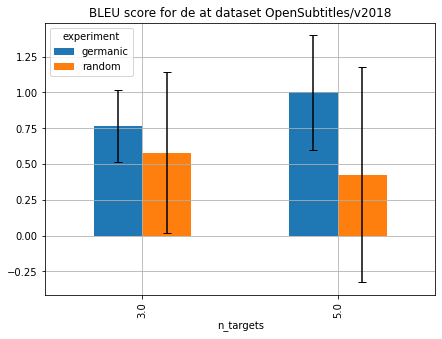
\includegraphics[width=0.48\textwidth]{../img/de_opensubtitles_13_1.png}
	}\hfill
	%\vspace*{\floatsep}% https://tex.stackexchange.com/q/26521/5764
	\subcaptionbox{MultiUn, bilingual score: 25.4 \acrshort{bleu}}[0.48\textwidth]{
		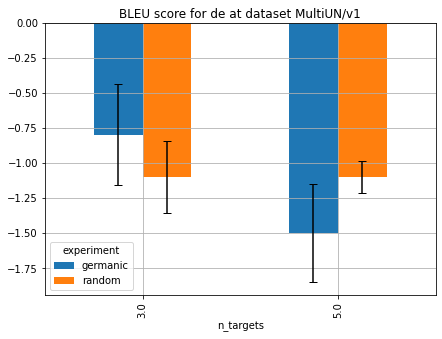
\includegraphics[width=0.48\textwidth]{../img/de_multiun_25_4.png}
	}

	\begin{minipage}{0.48\textwidth}
		\mycaption{En\to{}De \acrshort{bleu} score difference: Random vs. Germanic}{
			On \emph{X} axis - number of target languages.
			On \emph{Y} axis - difference score comparing with monolingual \acrshort{bleu}.
			Black vertical lines show standard deviation.
			(a) Adding random target language as well as a related one slightly
			improves German translation score on speech transcript.
			(b) Adding neither a random nor a related target language helps with
			prepared speeches transcripts and documents in German.
			(c) Adding a related target language into the mix introduces
			less new unique subwords.
		}
		\label{fig:de_random_vs_germanic}
	\end{minipage}\hfill
	\subcaptionbox{Subword dictionary size used for target side}[0.48\textwidth]{
		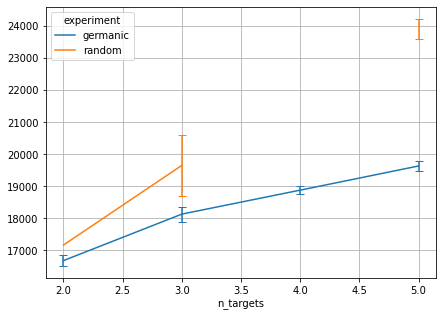
\includegraphics[width=0.48\textwidth]{../img/de_tgt_subwords.png}
	}\hfill
	\vspace*{\floatsep}% https://tex.stackexchange.com/q/26521/5764

\end{figure}

\begin{figure}[h]

	\centering
	\subcaptionbox{OpenSubtitles/v2018, bilingual score: 15.6 \acrshort{bleu}}[0.48\textwidth]{
		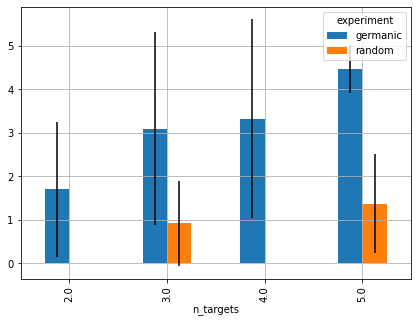
\includegraphics[width=0.48\textwidth]{../img/da_opensubtitles_15_6.png}
	}\hfill
	\subcaptionbox{Europarl/v3, bilingual score: 24.6 \acrshort{bleu}}[0.48\textwidth]{
		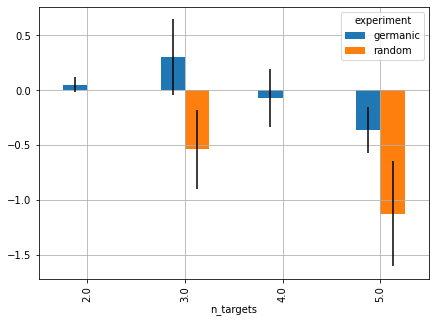
\includegraphics[width=0.48\textwidth]{../img/da_europarl_24_6.png}
	}\hfill
	%\vspace*{\floatsep}% https://tex.stackexchange.com/q/26521/5764
	\subcaptionbox{Subword dictionary size used for target side}[0.48\textwidth]{
		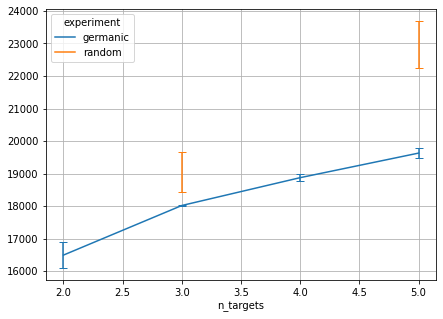
\includegraphics[width=0.48\textwidth]{../img/da_tgt_subwords.png}
	}\hfill
	\begin{minipage}{0.48\textwidth}
	\mycaption{En\to{}Da \acrshort{bleu} score difference: Random vs. Germanic}{
		Axis are same as above.
		(a) For OpenSubtitles test set which which consists of human speech transcripts
		adding similar target language to the mix significantly imporves the result.
		(b) For Europarl/v3 which consists of prepared speeches transcripts and documents
		adding more germanic languages to the mix did not worsened Danish translation
		quality unlike the case with German.
		(c) Adding random target language to the mix adds more subwords to the target
		subword dictionary
	}
	\label{fig:da_random_vs_germanic}
	\end{minipage}
\end{figure}


\cleardoublepage
\subsection{Slavic with cyrillic script}
\label{subsection:cyrillic_group}

Here \textit{Slavic with cyrillic script} group consists of
Bulgarian, Macedonian, Russian and Ukrainian.
Models En\to{}Cyrillic are compared to En\to{}non-Cyrillic, where non-Cyrillic consists
of any langauge except from those from the group above.
On Figures \ref{fig:bg_random_vs_cyrillic} and \ref{fig:ru_random_vs_cyrillic} some selected
results are visualized along with vocabulary changes. Test sets for subfigures (a) and (b)
selected the same way as in \ref{subsection:germanic_group}.

From the two opposite observations of \ref{subsection:germanic_group} in this case
the second one is observed: low results are getting slightly better,
good results are getting slightly or significantly worse.

\begin{figure}[h]

	\centering
	\subcaptionbox{OpenSubtitles/v2018, bilingual score: 23.7 \acrshort{bleu}}[0.48\textwidth]{
		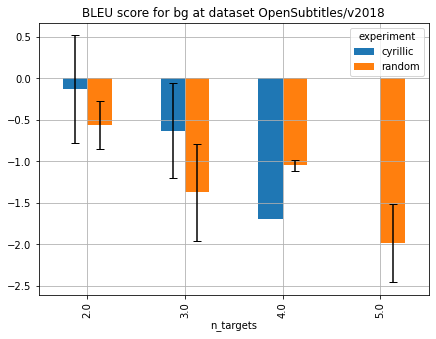
\includegraphics[width=0.48\textwidth]{../img/bg_opensubtitles_23_7.png}
	}\hfill
	\subcaptionbox{Europarl/v3, bilingual score: 41.4 \acrshort{bleu}}[0.48\textwidth]{
		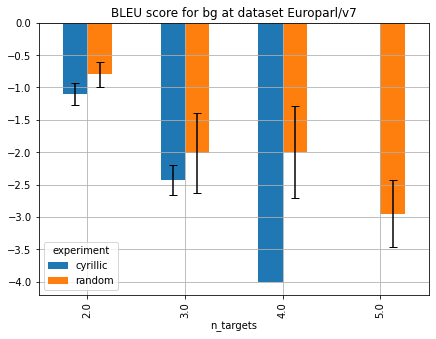
\includegraphics[width=0.48\textwidth]{../img/bg_europarl_41_4.png}
	}\hfill
	%\vspace*{\floatsep}% https://tex.stackexchange.com/q/26521/5764
	\subcaptionbox{Subword dictionary size used for target side}[0.48\textwidth]{
		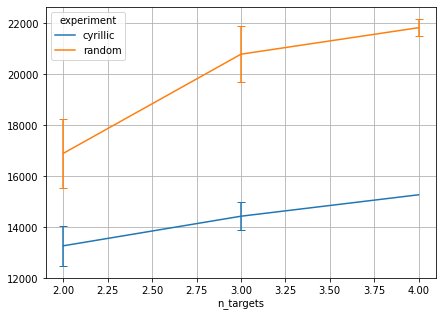
\includegraphics[width=0.48\textwidth]{../img/bg_tgt_subwords.png}
	}\hfill
	\begin{minipage}{0.48\textwidth}
	\mycaption{En\to{}Bg \acrshort{bleu} score difference: Random vs. Slavic with cyrillic script}{
		Axis are same as for Figures \ref{fig:da_random_vs_germanic}
		and \ref{fig:de_random_vs_germanic}. There is not any data for Cyrillic and
		5 targets as there are only 4 such languages in the en-to-36 dataset.
		Both (a) and (b) show significant decrease in translation quality. On (c)
		it is clearly visible how adding a random language with non-cyrillic script
		increases target subword vocabulary size.
	}
	\label{fig:bg_random_vs_cyrillic}
	\end{minipage}
\end{figure}

\begin{figure}[h]

	\centering
	\subcaptionbox{OpenSubtitles/v2018, bilingual score: 19.2 \acrshort{bleu}}[0.48\textwidth]{
		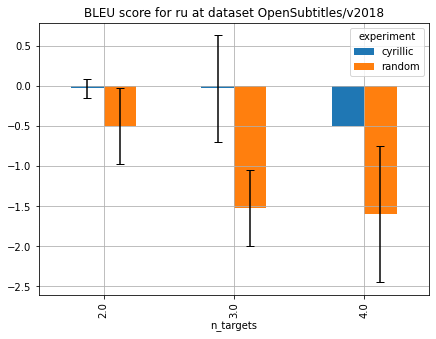
\includegraphics[width=0.48\textwidth]{../img/ru_opensubtitles_19_2.png}
	}\hfill
	\subcaptionbox{MultiUN, bilingual score: 14.6 \acrshort{bleu}}[0.48\textwidth]{
		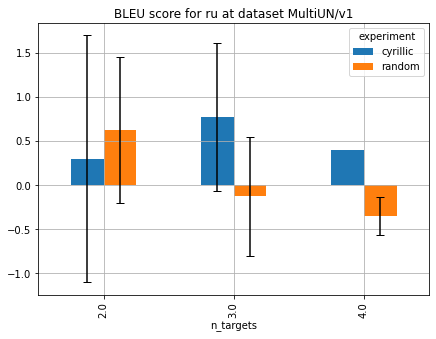
\includegraphics[width=0.48\textwidth]{../img/ru_multiun_14_6.png}
	}\hfill
	%\vspace*{\floatsep}% https://tex.stackexchange.com/q/26521/5764
	\subcaptionbox{Subword dictionary size used for target side}[0.48\textwidth]{
		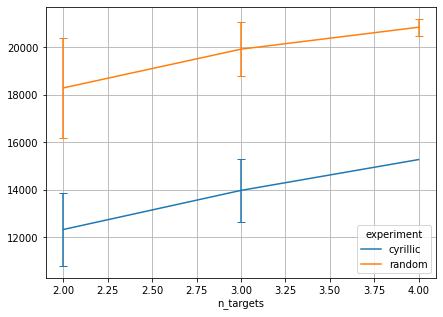
\includegraphics[width=0.48\textwidth]{../img/ru_tgt_subwords.png}
	}\hfill
	\begin{minipage}{0.48\textwidth}
	\mycaption{En\to{}Ru \acrshort{bleu} score difference: Random vs. Slavic with cyrillic script}{
		Axis are same as for Figures \ref{fig:da_random_vs_germanic},
		\ref{fig:de_random_vs_germanic} and \ref{fig:bg_random_vs_cyrillic}.
		There is not any data for Cyrillic and
		5 targets as there are only 4 such languages in the en-to-36 dataset.
		Both (a) and (b) show significant decrease in translation quality. On (c)
		it is clearly visible how adding a random language with non-cyrillic script
		increases target subword vocabulary size.
	}
	\label{fig:ru_random_vs_cyrillic}
	\end{minipage}
\end{figure}

%\begin{table}[h]
%\begin{subtable}[t]{1\linewidth}
%\begin{tabular}{rrrrrrr}
%\toprule
%n\_targets & \multicolumn{2}{l}{mean} & \multicolumn{2}{l}{count} & \multicolumn{2}{l}{std} \\
%          &   cyrillic &   random & cyrillic & random &  cyrillic &    random \\
%\midrule
%        2 &  14.950000 &  15.2625 &      6.0 &    8.0 &  1.209545 &  0.757699 \\
%        3 &  15.383333 &  14.5625 &      6.0 &    8.0 &  0.725029 &  0.616297 \\
%        4 &  15.200000 &  14.2750 &      2.0 &    4.0 &  0.282843 &  0.206155 \\
%\bottomrule
%\end{tabular}
%\caption{MultiUN/v1}
%\label{table:ru/multi_un}
%\end{subtable}
%\begin{subtable}[t]{1\linewidth}
%\begin{tabular}{rrrrrrr}
%\toprule
%n\_targets & \multicolumn{2}{l}{mean} & \multicolumn{2}{l}{count} & \multicolumn{2}{l}{std} \\
%          &   cyrillic &  random & cyrillic & random &  cyrillic &    random \\
%\midrule
%        2 &  22.883333 &  22.875 &      6.0 &    8.0 &  0.507609 &  0.514782 \\
%        3 &  22.333333 &  21.050 &      6.0 &    8.0 &  0.273252 &  0.705084 \\
%        4 &  21.050000 &  20.950 &      2.0 &    4.0 &  0.494975 &  0.465475 \\
%\bottomrule
%\end{tabular}
%\caption{NewsCommentary/v11}
%\label{table:ru/news_v11}
%\end{subtable}
%\begin{subtable}[t]{1\linewidth}
%\begin{tabular}{rrrrrrr}
%\toprule
%n\_targets & \multicolumn{2}{l}{mean} & \multicolumn{2}{l}{count} & \multicolumn{2}{l}{std} \\
%          &   cyrillic &   random & cyrillic & random &  cyrillic &    random \\
%\midrule
%        2 &  19.266667 &  18.7375 &      6.0 &    8.0 &  0.273252 &  0.396187 \\
%        3 &  19.350000 &  17.7875 &      6.0 &    8.0 &  0.653452 &  0.418970 \\
%        4 &  18.900000 &  17.5750 &      2.0 &    4.0 &  0.282843 &  0.613052 \\
%\bottomrule
%\end{tabular}
%\caption{OpenSubtitles/v2018}
%\label{table:ru/news_v11}
%\end{subtable}
%\caption{Mean \acrshort{bleu} score, its standard deviation and number of trained models (count) for Russian at various datasets}
%\end{table}
%
%
%
%\begin{table}[h]
%\begin{subtable}[t]{1\linewidth}
%\begin{tabular}{rrrrrrr}
%\toprule
%n\_targets & \multicolumn{2}{l}{mean} & \multicolumn{2}{l}{len} & \multicolumn{2}{l}{std} \\
%          &   cyrillic &     random & cyrillic & random &  cyrillic &    random \\
%\midrule
%        2 &  40.433333 &  40.683333 &      6.0 &    6.0 &  0.273252 &  0.183485 \\
%        3 &  39.216667 &  39.506250 &      6.0 &   16.0 &  0.318852 &  0.611521 \\
%        4 &  37.750000 &  39.450000 &      2.0 &    4.0 &  0.494975 &  0.525991 \\
%        5 &        NaN &  38.483333 &      NaN &   12.0 &       NaN &  0.511386 \\
%\bottomrule
%\end{tabular}
%\caption{Europarl/v7}
%\label{ table:bg/Europarl/v7 }
%\end{subtable}
%\begin{subtable}[t]{1\linewidth}
%\begin{tabular}{rrrrrrr}
%\toprule
%n\_targets & \multicolumn{2}{l}{mean} & \multicolumn{2}{l}{len} & \multicolumn{2}{l}{std} \\
%          &   cyrillic &     random & cyrillic & random &  cyrillic &    random \\
%\midrule
%        2 &  23.683333 &  23.250000 &      6.0 &    6.0 &  0.598052 &  0.225832 \\
%        3 &  23.216667 &  22.406250 &      6.0 &   16.0 &  0.470815 &  0.619106 \\
%        4 &  22.300000 &  22.600000 &      2.0 &    4.0 &  0.424264 &  0.081650 \\
%        5 &          - &  21.741667 &        - &   12.0 &         - &  0.494439 \\
%\bottomrule
%\end{tabular}
%\caption{OpenSubtitles/v2018}
%\label{tab:bg/OpenSubtitles/v2018}
%\end{subtable}
%\caption{\acrshort{bleu} score for Bulgarian at various datasets }
%\end{table}
%
%\begin{table}[]
%\begin{tabular}{r|rr|cc|rr}
%\toprule
%n\_targets & \multicolumn{2}{c}{mean} & \multicolumn{2}{c}{count} &\multicolumn{2}{c}{std} \\
%          &   cyrillic &  random & cyrillic & random &  cyrillic &    random \\
%\midrule
%        1 & \multicolumn{2}{c|}{41.40} & \multicolumn{2}{c|}{1} & \multicolumn{2}{c}{-}  \\
%\midrule
%        2 &         40.30 &      40.60 &           3 &        3 &       0.17 &      0.20 \\
%        3 &         38.97 &      39.39 &           3 &        8 &       0.23 &      0.62 \\
%        4 &         37.40 &      39.40 &           1 &        2 &        --  &      0.71 \\
%        5 &           --  &      38.45 &         --  &        6 &        --  &      0.52 \\
%\bottomrule
%\end{tabular}
%
%\caption{\acrshort{bleu} score for  bg at dataset Europarl/v7 }
%\label{ table:bg/Europarl/v7 }
%\end{table}

%%% \cleardoublepage
%%% \section{Selecting target languages by linguistic similarity}

